\documentclass[a4paper,12pt]{article}
\usepackage[utf8]{inputenc}
\usepackage[spanish]{babel}
\usepackage{amsmath}
\usepackage{graphicx}
\usepackage{tocbibind}
\usepackage{hyperref}
% \usepackage{cite}

% \title{Linus Torvalds y el desarrollo de Linux}
% \author{José Antonio Concepción Alvarez\\  José Miguel Zayas Pérez \\ Grupo: 411 y 412}
% \date{\today}

\begin{document}

% Portada
% \maketitle

\begin{titlepage}
    \centering
    
    % Incluir la imagen
    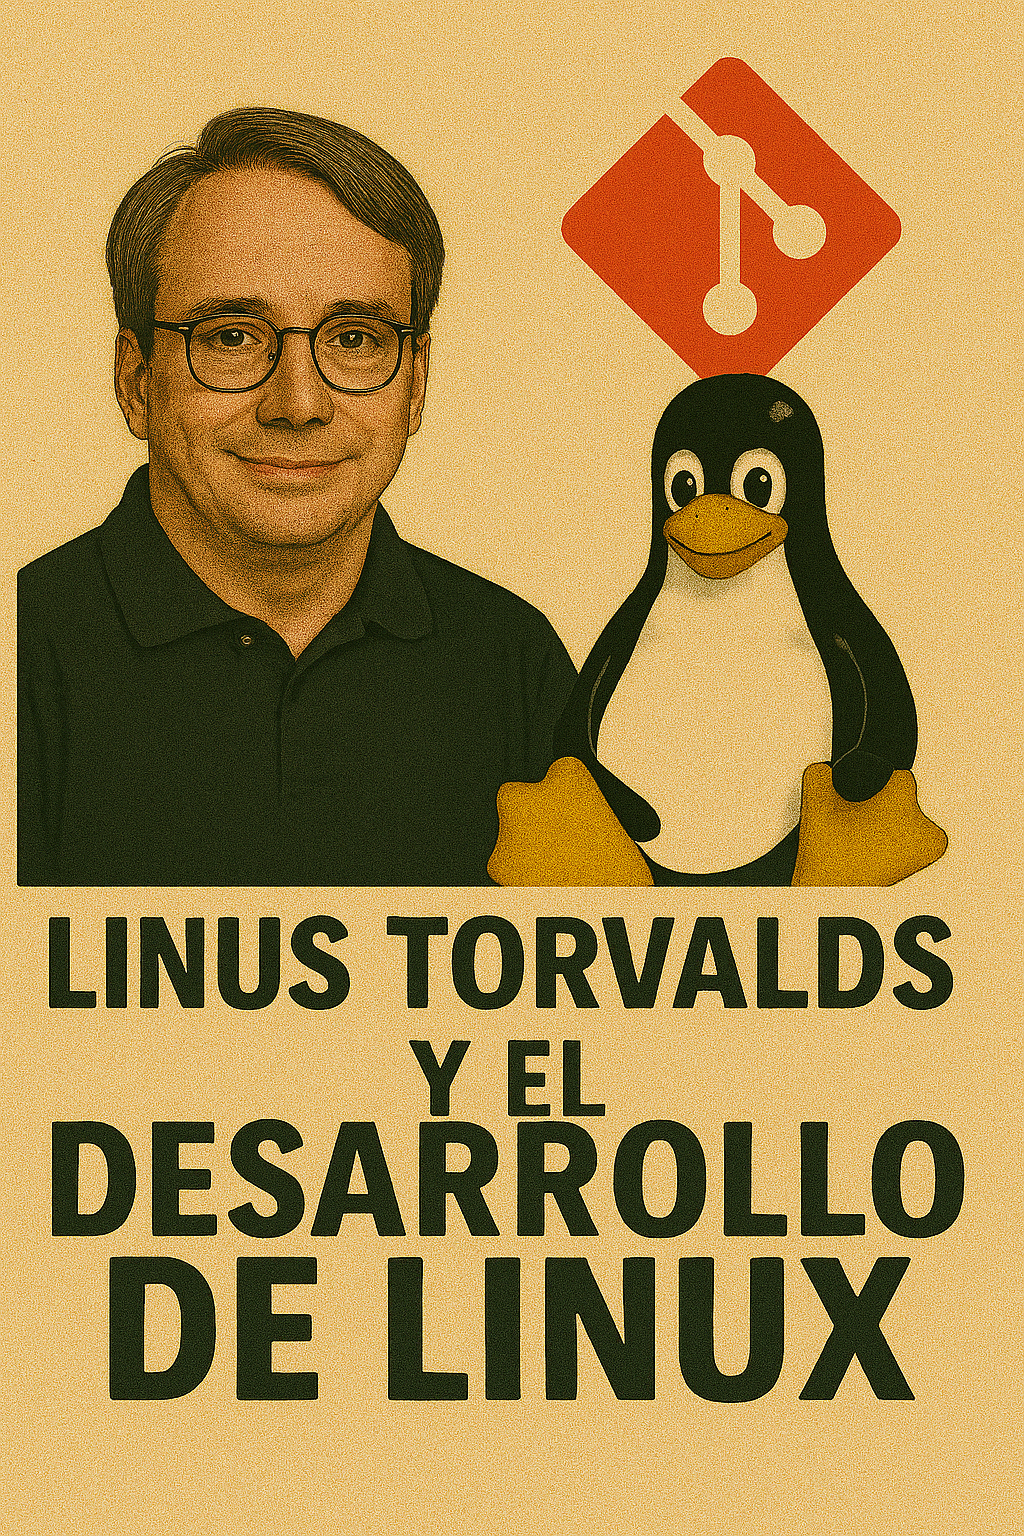
\includegraphics[width=1.0\textwidth]{images/front.png} % Cambia la ruta a la ubicación de tu imagen
    
    \vspace{1cm}
    \newpage
    
    % Título
    {\Huge \textbf{Linus Torvalds y el desarrollo de Linux}}\\
    \vspace{0.5cm}
    
    % Autores
    {\Large José Antonio Concepción Alvarez \\  José Miguel Zayas Pérez \\ Grupo: 411 y 412}
    
    % \vfill
    
    % Fecha
    % {\large \today}
   \thispagestyle{empty} 
\end{titlepage}

\begin{centering}
    \vspace{2cm}
    \textbf{Resumen}\\
    Este ensayo explora la vida y las contribuciones de Linus Torvalds, el
    creador del núcleo Linux y Git, y su impacto en la historia de la
    computación. Se presenta un análisis de su relevancia en el desarrollo del
    software libre y de código abierto, destacando cómo su trabajo ha
    transformado el desarrollo colaborativo en la industria del software. A
    través de un examen de los antecedentes históricos, el nacimiento y
    evolución de Linux, y su influencia en la infraestructura de internet y
    dispositivos móviles, se argumenta que la influencia de Torvalds va más allá
    de la creación de software, abarcando un legado de colaboración y
    transparencia en el desarrollo tecnológico. Finalmente, se reflexiona sobre
    su impacto en el futuro de la tecnología y la filosofía del código abierto.
\end{centering}
\newpage

% Índice
\tableofcontents
\newpage

% Sección 1
\section{Introducción} 

En la vasta cronología de la historia de la computación, pocos nombres han
dejado una huella tan profunda y duradera como el de Linus Torvalds. Reconocido
mundialmente como el creador del núcleo del sistema operativo Linux y del
sistema de control de versiones distribuido Git, Torvalds ha sido una figura
clave en la evolución del software moderno. Su obra no solo ha influido en la
infraestructura tecnológica global, sino que también ha catalizado una
transformación en la manera en que el software es desarrollado, compartido y
perfeccionado.

El núcleo Linux, iniciado como un proyecto personal en 1991, se ha convertido en
el corazón de millones de sistemas, desde servidores y supercomputadoras hasta
dispositivos móviles. A su vez, Git, concebido inicialmente para gestionar el
desarrollo del propio kernel de Linux, se ha posicionado como la herramienta
estándar para el control de versiones en proyectos de cualquier escala. Sin
embargo, más allá de estos hitos técnicos, la relevancia de Torvalds se extiende
a un plano más amplio: su trabajo ha redefinido las dinámicas del desarrollo
colaborativo, sentando las bases del movimiento de código abierto y fomentando
una cultura de cooperación, transparencia y meritocracia técnica.

Este trabajo abordará la influencia de Linus Torvalds en el desarrollo de
software, el crecimiento de la comunidad de Open Source, la colaboración a gran
escala y la consolidación de un modelo de innovación abierto que ha transformado
profundamente la industria tecnológica y la cultura digital contemporánea.  
\newpage

% Sección 2
\section{Antecedentes} 

\subsection{Sistemas Operativos antes de la llegada de Linux}
A finales del siglo XX, el panorama de los sistemas operativos estaba marcado
por una diversidad de plataformas que reflejaban tanto los avances tecnológicos
como las limitaciones económicas y de acceso al software. Entre ellos, UNIX,
lanzado en 1969, emergió como un pilar fundamental en entornos de alto
rendimiento. Para inicios de los años noventa, se había consolidado como el
sistema operativo dominante en supercomputadoras y servidores, siendo adoptado
por gigantes tecnológicos como IBM, Sun y Apple. No obstante, su alto costo y la
fragmentación en múltiples variantes —derivadas de la base de código de AT\&T
(System V) y de la Universidad de California-Berkeley (BSD)— lo convertían en
una opción inaccesible para la mayoría de los estudiantes y usuarios
particulares.

En paralelo, MS-DOS se convirtió en el estándar de facto en el mercado de
computadoras personales. Al ser incluido en casi todas las máquinas compatibles
con IBM, permitió a Microsoft alcanzar un dominio total en el mercado de
sistemas operativos hacia 1991, precisamente el año en que Linus Torvalds
publicó la primera versión de prueba del núcleo Linux. MS-DOS sirvió como el
vínculo crucial entre el hardware y el software, en una era anterior al auge de
las interfaces gráficas como Macintosh y Windows.

Antes de esta hegemonía de Microsoft, otro sistema operativo había tenido un
papel destacado: CP/M (Control Program for Microcomputers), desarrollado por
Digital Research. Popular entre las máquinas de 8 bits, CP/M se instaló en
millones de dispositivos, alcanzando un estimado de 200 millones de copias
vendidas. Sin embargo, su protagonismo fue efímero frente al crecimiento
explosivo de MS-DOS.

Aunque su relevancia había disminuido con la llegada de las
computadoras personales, los sistemas operativos de mainframe como OS/360 de
IBM, así como BOS y TOS, tuvieron una importancia notable en décadas anteriores,
especialmente en el ámbito corporativo y gubernamental, sentando muchas de las
bases conceptuales que influenciarían generaciones posteriores de software.

Para estudiantes y académicos, una alternativa fue MINIX, un sistema operativo
de código fuente abierto diseñado con fines educativos por Andrew S. Tanenbaum.
Fue precisamente utilizando MINIX en la Universidad de Helsinki que Linus
Torvalds identificó sus limitaciones y decidió iniciar el desarrollo de su
propio sistema operativo, con una arquitectura más robusta y eficiente. Su
proyecto fue anunciado inicialmente en un grupo de discusión de MINIX, marcando
el inicio de lo que se convertiría en uno de los mayores fenómenos del software
libre.


\subsection{El desarrollo de software hasta el momento}

Antes de la irrupción de Linux y el ascenso del movimiento de código abierto, el
desarrollo de software se encontraba fuertemente arraigado en un modelo cerrado
y comercial. El software propietario era la norma dominante: un sistema en el
que las empresas o individuos mantenían el control exclusivo del código fuente,
su distribución y su explotación económica. En esta lógica, el software era
considerado un producto sujeto a propiedad intelectual, cuya protección era
indispensable para asegurar su rentabilidad.

Una de las características esenciales del software propietario era precisamente
su naturaleza de código cerrado. Los usuarios podían adquirir licencias de uso,
pero solo accedían a binarios o código objeto, sin posibilidad de revisar,
modificar o adaptar el código fuente. Esta restricción limitaba tanto la
comprensión profunda del software como la capacidad colectiva para mejorarlo o
adaptarlo a nuevas necesidades.

El modelo se sustentaba en un esquema de comercialización y licenciamiento.
Empresas como Microsoft construyeron imperios bajo este enfoque, los sistemas
como MS-DOS dominaban el mercado de computadoras personales. Incluso soluciones
más potentes como UNIX, operaban bajo costosas licencias que reservaban el
acceso y las modificaciones a una élite corporativa o académica con recursos
suficientes.

El desarrollo en este contexto era interno y centralizado. Los equipos de
programación pertenecían a las propias empresas, y tanto la depuración como la
mejora de los productos eran procesos controlados y frecuentemente lentos y
costosos. La dependencia de recursos internos limitaba la velocidad de
innovación, dificultando la respuesta ágil a los cambios del entorno
tecnológico.

Durante los años 60, la creciente complejidad de los proyectos llevó a lo que se
conoció como la "crisis del software". Iniciativas como el sistema OS/360 de IBM
expusieron las dificultades de gestionar proyectos a gran escala, lo que impulsó
la búsqueda de metodologías más estructuradas para el desarrollo. Esta época
también vio un auge en el diseño de nuevos lenguajes de programación, destinados
a distintos nichos: COBOL y FORTRAN dominaron en la industria y la ciencia,
mientras que BASIC, desarrollado en Dartmouth, encontró un lugar central en las
primeras microcomputadoras. Pascal, introducido en 1971, se convirtió en un
lenguaje clave en la educación formal de programación.

Otro cambio técnico crucial de la época fue la introducción del `time-sharing´,
que permitió compartir el poder computacional de grandes máquinas entre
múltiples usuarios. Este paradigma impulsó el acceso a la computación en
entornos académicos y favoreció la difusión de lenguajes como BASIC, que
democratizaron el uso de la programación en los albores de la informática
personal.

En este entorno surgió UNIX, desarrollado en Bell Labs a partir de 1969. Su
portabilidad, eficiencia y adecuación para el`time-sharin´ lo convirtieron en el
sistema operativo preferido en universidades y centros de investigación, y más
tarde en servidores y supercomputadoras. Sin embargo, su costo y el carácter
cerrado de sus licencias lo mantuvieron alejado del usuario promedio.

En contraste con esta hegemonía comercial y cerrada, comenzaban a emerger
comunidades que compartían software libremente, como la del Laboratorio de
Inteligencia Artificial del MIT. El desencanto con las restricciones del
software propietario llevó a figuras como Richard Stallman a iniciar un
movimiento en defensa de la libertad del usuario. En 1985 fundó la Free Software
Foundation y lanzó el proyecto GNU, cuyo objetivo era construir un sistema
operativo completamente libre, compatible con UNIX. Stallman consideraba el
secretismo del código como un atentado contra el conocimiento colectivo.
Paralelamente, iniciativas como la Berkeley Software Distribution (BSD) ofrecían
versiones abiertas de UNIX, sentando precedentes fundamentales para el
desarrollo posterior de Linux.

\subsection{Las universidades y cuestiones filosóficas}
Las universidades desempeñaron un papel crucial en el desarrollo del software,
especialmente en sus inicios, donde profesores y estudiantes universitarios
fueron actores clave en el movimiento del software libre. En la década de 1970,
muchas universidades lideraban proyectos de programación y vendían sus
resultados, adoptando políticas que promovían la publicación de software como
libre bajo la licencia GPL. Por ejemplo, el laboratorio de programación de
Harvard no permitía la instalación de programas cuyo código fuente no estuviera
disponible públicamente. Además, los gobiernos financiaron proyectos de
desarrollo de software, como el compilador GNU Ada, desarrollado por la
Universidad de Nueva York con fondos de las Fuerzas Aéreas de EE. UU., con la
condición de que el código se donara a la Free Software Foundation. Sin embargo,
las políticas gubernamentales de control de exportaciones y leyes como la DMCA
(Digital Millennium Copyright Act) podían restringir la distribución de software
libre a nivel internacional.

Los códigos fuente cerrados generaban frustración entre los usuarios, ya que les
impedían aprender del software y corregir errores, así como adaptar el software
a necesidades específicas. Un problema común de la época es que las instituciones,
no podían modificar un software comercial por falta de acceso al código fuente,
lo que resultaba en meses de trabajo innecesario. Además, la existencia de
software propietario obstaculizaba la evolución natural del software, ya que
obligaba a los desarrolladores a comenzar desde cero en lugar de modificar
programas existentes. Esto también dificultaba el aprendizaje de nuevos
programadores, quienes no podían estudiar el código fuente de programas
complejos. En ese contexto, sistemas operativos como el Sistema Incompatible de
Uso Compartido (ITS) del MIT, escritos en lenguaje Assembler, eran dependientes
de arquitecturas específicas y se volvían obsoletos cuando estas dejaban de
fabricarse. 

Desde una perspectiva filosófica, el surgimiento del movimiento del software
libre representó mucho más que una simple alternativa técnica: fue una postura
ética frente a la estructura dominante del desarrollo informático. Tras décadas
de hegemonía del software propietario, donde el conocimiento era celosamente
guardado y la colaboración entre usuarios vista como una amenaza, emergió una
crítica profunda al modelo que convertía el software en un bien cerrado y
restrictivo. Richard Stallman y los primeros defensores del software libre
denunciaban que ocultar el código fuente era no solo injusto, sino inmoral,
llegando a calificarlo como un pecado y un crimen contra la humanidad". En este
marco, el software libre no se trataba meramente de gratuidad, sino de libertad:
libertad para estudiar, modificar, compartir y construir colectivamente. Frente
a la narrativa empresarial que equiparaba compartir con piratería, el movimiento
proponía una ética de cooperación, de empoderamiento del usuario y de
construcción social del conocimiento. Rechazando el aislamiento al que condenaba
el software propietario, esta filosofía rescataba la dimensión humana de la
tecnología, defendiendo el derecho de las personas a controlar las herramientas
que median su vida digital. Así, el software libre planteaba una alternativa
civilizatoria: una tecnología al servicio de la libertad, no del control.

\subsection{El usuario final}
La relación entre el usuario final y el software, en el contexto del modelo
propietario, fue marcada por la exclusión, la dependencia y la pasividad. En
este modelo dominante antes de la irrupción del software libre, el usuario era
un receptor pasivo del producto, sin derecho ni posibilidad de intervenir en su
funcionamiento interno. El código cerrado —la práctica de distribuir software
únicamente en forma de binarios ejecutables, sin acceso al código fuente—
impidió que los usuarios comprendieran, adaptaran o mejoraran los programas que
usaban. Esta opacidad no solo restringía el aprendizaje técnico, sino que
reforzaba una barrera entre quien produce conocimiento tecnológico y quien
simplemente lo consume.

El usuario, por tanto, no era un colaborador ni un co-creador del software, sino
un consumidor subordinado a las decisiones del proveedor. Las licencias de uso
establecían los términos en los que se podía operar el software, negando
explícitamente la redistribución, modificación o copia. Esta situación
consolidaba una relación unidireccional, donde el proveedor centralizaba el
poder técnico y comercial, y el usuario quedaba relegado a un rol de obediencia
operativa. Incluso en casos en que el usuario —como una institución bancaria—
requería una modificación funcional específica, la ausencia de acceso al código
fuente lo condenaba a depender del proveedor o a incurrir en procesos costosos y
prolongados.

Además, la relación se caracterizaba por una fuerte dependencia técnica y
económica: si surgía un error o necesidad, el usuario debía esperar a que el
proveedor respondiera. Y si esa necesidad no era considerada rentable,
simplemente se ignoraba. Esta lógica instrumental convirtió al software en una
herramienta cerrada y rígida, en lugar de una plataforma adaptable o
personalizable.

Más profundamente, el modelo propietario fomentó una relación de alienación
entre el usuario y el software: se utilizaba, pero no se comprendía; se confiaba
en él, pero no se podía transformar. En este contexto, la figura del usuario
como agente activo del conocimiento era anulada. Cualquier intento de compartir
o adaptar software era estigmatizado como "piratería", borrando las nociones de
solidaridad y cooperación que habían caracterizado los primeros entornos
académicos de programación.

Este escenario de restricciones, dependencia y exclusión fue el caldo de cultivo
ideal para que un joven Linus Torvalds —frustrado por las limitaciones de los
sistemas existentes como MINIX y motivado por una visión más abierta del
desarrollo tecnológico— iniciara en 1991 el proyecto que daría origen a Linux.
En un contexto dominado por el control propietario y la pasividad del usuario,
su propuesta representó un giro radical hacia la colaboración, la transparencia
y la libertad en el uso del software.

% Sección 3
\section{El Nacimiento y Evolución de Linux} 
- El desarrollo inicial de Linux
como un proyecto personal.\\ 
- La transición de Linux a un proyecto colaborativo
global.\\ 
- El impacto de la Licencia Pública General de GNU (GPL) en la
expansión de Linux.\\ 
- La evolución de Linux y su adopción en servidores,
dispositivos móviles y sistemas embebidos.

% Sección 4
\section{El Impacto de Linux en la Industria de la Computación} 
- La influencia
de Linux en el desarrollo de servidores y la infraestructura de internet.\\ 
- El
papel de Linux en la revolución de los dispositivos móviles a través de
Android.\\ 
- La adopción de Linux en supercomputadoras y sistemas de alto
rendimiento.\\ 
- El impacto económico y social de Linux.

% Sección 5
\section{Linus Torvalds y el Desarrollo Colaborativo}

\subsection{Una nueva forma}

Cómo hemos visto, Linux fue principalmente un proyecto personal de Linus Torvalds.
Comenzó a trabajar en el kernel como un hobby, sin la intención de competir con
sistemas comerciales como UNIX ni de desarrollar algo tan ambicioso como GNU. Su
objetivo inicial era simplemente crear un sistema operativo funcional que
pudiera utilizar en su propia computadora y, de paso, ayudar a otros
estudiantes.

Un aspecto fundamental de la organización inicial del proyecto fue su apertura
al público desde el primer momento. Torvalds anunció su trabajo en un grupo de
noticias del sistema operativo MINIX, invitando a otros usuarios a probar su
sistema y a ofrecer comentarios. Esta transparencia y disposición a recibir
retroalimentación contrastaban fuertemente con los modelos de desarrollo
tradicionales, que solían mantenerse en secreto durante sus fases tempranas.

Otro elemento clave fue la decisión de licenciar Linux bajo la GNU General
Public License (GPL). Esta licencia permitía a cualquier persona usar, modificar
y distribuir el código fuente de Linux de forma libre. Fue una decisión
estratégica que atrajo a una comunidad creciente de desarrolladores, quienes
comenzaron a colaborar en el proyecto de manera voluntaria y entusiasta,
cimentando las bases del ecosistema de software libre que conocemos hoy.

La organización del desarrollo en sí misma era inicialmente muy informal y sin
una jerarquía estricta. No había una estructura de gestión tradicional con jefes
supervisando a los desarrolladores. Cada miembro de la comunidad tenía derecho a
voz y voto, y sus propuestas eran consideradas. Sin embargo, Linus Torvalds se
mantuvo como la figura central, tomando las decisiones finales sobre qué se
incluía, eliminaba o cambiaba en el núcleo/kernel. Esta figura de `general'
surgió, según el propio Torvalds, para evitar conflictos y asegurar la
eficiencia del desarrollo.  Con el tiempo, surgieron roles más definidos de
manera orgánica dentro de la comunidad. Un "consejo de ancianos" se formó,
compuesto por desarrolladores clave como Dave Miller, responsable de la calidad
del código; Ted Ts'o, encargado de las relaciones públicas y la difusión de
Linux; y Alan Cox, considerado la mano derecha de Torvalds para aspectos
importantes de la estructura del núcleo.

Podemos señalar además algunos contrastes con respecto a los modelos existentes:

\begin{itemize}
    \item \textbf{Desarrollo centralizado vs. desarrollo distribuido:} 
        Los modelos tradicionales, como los utilizados por Microsoft en el
        desarrollo de Windows, se basaban en pequeños equipos de programadores
        internos que trabajaban en un código cerrado. Linux, en cambio, se
        desarrolló de manera distribuida con la colaboración de cientos e
        incluso miles de personas de todo el mundo.
    \item \textbf{Motivación económica vs. motivación comunitaria:}  En los
    modelos tradicionales, los desarrolladores generalmente trabajaban por una
    recompensa económica directa. En el inicio de Linux, muchos contribuyeron
    voluntariamente, motivados por el respeto de sus colegas y el deseo de
    mejorar el software.
    \item \textbf{Desarrollo planificado vs. desarrollo evolutivo:} Los modelos
    tradicionales a menudo seguían un plan de desarrollo rígido, similar a un
    proyecto de construcción. El desarrollo de Linux fue mucho más orgánico y
    evolutivo, creciendo y mejorando gracias a las contribuciones de la comunidad.
\end{itemize}

Todos estos mecanismos permitieron programadores de todo el mundo colaboraran eficazmente en el proyecto Linux.

\subsection{Linus, líder técnico y coordinador}
Aunque el proyecto se caracterizó por su desarrollo distribuido y la
colaboración de miles de programadores voluntarios de todo el mundo, Torvalds
siempre mantuvo la autoridad final sobre el kernel de Linux.
u profundo conocimiento del sistema le permitió dirigir su desarrollo y tomar
decisiones técnicas cruciales. Incluso con el crecimiento masivo del proyecto,
Torvalds se mantuvo como la única persona autorizada para fusionar las
contribuciones al proyecto principal. Esto le permitía seleccionar las mejores
ideas, decidir qué incluir, eliminar o modificar en el núcleo/kernel. 
Aunque no existía una jerarquía estricta dentro de la comunidad, Torvalds se
convirtió en la figura central en quien la comunidad confiaba más. Su estilo de
liderazgo se describió como el de un `dictador benevolente', un término que
sugiere que mantenía el control final para asegurar la coherencia y dirección
del proyecto, pero lo hacía con el consenso y el respeto de la comunidad. Según
el propio Torvalds, su método para gestionar el proyecto con cientos de miles de
desarrolladores era esperar a que la gente se ofreciera voluntariamente para
hacerse cargo de diferentes subsistemas, en lugar de delegar proactivamente.

\subsection{Problemas con BitKeeper, el surgimiento de Git}

A medida que más programadores se unían al proyecto Linux y comenzaban a
contribuir con mejoras y correcciones, la tarea de revisar y gestionar todas
estas aportaciones se volvió cada vez más compleja. En un principio, Linus
Torvalds administraba el flujo de contribuciones principalmente a través del
correo electrónico, lo cual funcionaba mientras el volumen de cambios era
manejable. Sin embargo, con el crecimiento exponencial de la comunidad, se hizo
evidente la necesidad de una herramienta más eficiente.

La escala y la naturaleza distribuida del desarrollo del kernel de Linux exigían
un sistema de control de versiones más robusto que los disponibles en ese
momento.

Antes de la creación de Git, los sistemas de control de versiones más utilizados
eran mayoritariamente centralizados. Herramientas como Concurrent Versions
System (CVS) y Subversion (SVN) dominaban el panorama, sustentadas en un modelo
donde un único repositorio central albergaba todo el historial de cambios.
Aunque estos sistemas funcionaban de forma aceptable en entornos de equipos
pequeños o proyectos simples, se mostraban deficientes al escalar hacia
proyectos complejos, distribuidos y de rápida evolución como el kernel de Linux.

Los sistemas de control de versiones centralizados presentaban serias
limitaciones: dependían de un único servidor (punto crítico de fallo), ofrecían
bajo rendimiento en operaciones clave, complicaban la resolución de conflictos
entre desarrolladores y no permitían trabajar sin conexión. Estas deficiencias
resultaron inviables para proyectos complejos y distribuidos como el kernel de
Linux, que requerían una infraestructura más ágil, descentralizada y robusta.

Antes de 2002, Linus Torvalds no utilizaba ninguna herramienta formal de control
de versiones (SCM) para el desarrollo del kernel de Linux. Aunque existían
opciones como CVS y Subversion, decidió no adoptarlas debido a sus limitaciones.
Sin embargo, a medida que el proyecto crecía y se volvía
más complejo, la comunidad de desarrolladores del kernel insistía en la
necesidad de una herramienta que facilitara la gestión del código.

Es por esto que, en 2002, surge la alianza con BitKeeper, una alternativa descentralizada
aunque de código propietario, que permitía a cada desarrollador tener una copia
completa del historial del proyecto y trabajar de forma local, mejorando
significativamente la eficiencia y autonomía del equipo, aunque a costa de
depender de una herramienta cerrada cuya licencia gratuita resultaría temporal y
conflictiva.

Desde el punto de vista tecnológico, BitKeeper era una herramienta ideal para el
desarrollo del kernel de Linux: distribuida, rápida y eficiente. Sin embargo, no
era software libre, lo que generó fuertes tensiones dentro de la comunidad.
Aunque Linus Torvalds valoraba su funcionalidad y había decidido adoptarlo,
enfrentó una creciente oposición por parte del núcleo del equipo del kernel, que
rechazaba depender de una herramienta propietaria.

Sin embargo, la relación entre la comunidad del software libre y BitMover era
tensa desde el inicio, ya que BitKeeper era un software propietario. Aunque
ofrecía licencias gratuitas para uso no comercial en proyectos de código
abierto, esta concesión era frágil. En 2005, tras una serie de desacuerdos,
BitMover decidió retirar el acceso libre a BitKeeper para los desarrolladores
del kernel de Linux. Este evento dejó a la comunidad sin una herramienta viable
para gestionar el desarrollo del proyecto.

Ante la retirada de la licencia gratuita por parte de BitMover y la presión
interna, Torvalds —a pesar de no querer realmente hacerlo— tomó la decisión de
crear su propia herramienta. En apenas dos semanas, desarrolló y lanzó Git, al
que describió con humor como “el estúpido rastreador de contenidos” (“the stupid
content tracker”), destacando su enfoque pragmático, minimalista y
descentralizado, en contraposición a las soluciones complejas y cerradas que
había conocido hasta entonces.

Fue en este contexto que Linus Torvalds diseñó y creó Git, un sistema de control
de versiones distribuido, rápido, escalable y completamente libre. Git no solo
solucionaba los problemas que habían afectado al desarrollo del kernel durante
años, sino que también establecía un nuevo estándar técnico y filosófico para la
colaboración en línea. Su arquitectura descentralizada, su manejo eficiente de
ramas y fusiones, y su integración fluida con el trabajo colaborativo hicieron
que Git se convirtiera rápidamente en el pilar de la infraestructura de
desarrollo moderno.


\subsection{La adopción masiva de Git}

Git terminó siendo tan increíblemente bueno en comparación con otros sistemas de control de
versiones que acabó comiéndose todo el mercado y teniendo una entidad propia y
muy reconocida. Antes de su aparición, no existía un flujo de trabajo
estandarizado en el mundo del software libre: cada proyecto y cada equipo
utilizaba sus propias herramientas, convenciones y procesos, lo que generaba una
auténtica "cacofonía" organizativa. En este contexto, Git no solo aportó una
solución técnica robusta, rápida y distribuida, sino que también instauró una
forma más estructurada y eficiente de colaborar en grandes comunidades,
transformando radicalmente la manera en que se desarrollaba software en todo el
mundo.

Git terminaría generando su mayor impacto a escala global cuando en 2008 se funda 
la plataforma GitHub. Su impacto fue profundo y multifacético, entre sus principales 
aportes se encuentran:

\begin{itemize}
    \item \textbf{Estandarización del flujo de trabajo:} GitHub consolidó la
    colaboración en una única plataforma durante el auge de la Web 2.0. Antes de
    su existencia, los proyectos usaban listas de correo y archivos comprimidos
    (tarballs) para compartir código, con procesos de colaboración poco
    uniformes. GitHub integró herramientas clave como gestión de issues,
    perfiles de contributores y pull requests, facilitando un flujo de trabajo
    limpio, transparente y colaborativo, accesible mediante una interfaz
    intuitiva.

    \item \textbf{Facilitación de la colaboración distribuida:} Al basarse en
    Git —el sistema de control de versiones distribuido creado por Linus
    Torvalds— GitHub permitió una colaboración verdaderamente descentralizada.
    Su plataforma hizo que Git fuese accesible incluso para desarrolladores sin
    experiencia previa, convirtiéndose rápidamente en el estándar de facto para
    el trabajo colaborativo a gran escala.

    \item \textbf{Visibilidad y descubrimiento de proyectos:} GitHub centralizó
    el ecosistema del código abierto, permitiendo a los usuarios descubrir
    nuevos proyectos y evaluar la reputación de sus contribuidores. Funciones
    como las estrellas ofrecieron indicadores simples de popularidad y calidad,
    impulsando la visibilidad y el crecimiento de iniciativas prometedoras.

    \item \textbf{Promoción de licencias permisivas:} GitHub también popularizó
    el uso de licencias abiertas como MIT y Apache, promoviendo una mayor
    reutilización del código. Esta tendencia contrastó con la filosofía más
    estricta del copyleft, ampliando el alcance del software libre y facilitando
    su adopción en contextos empresariales.

    \item \textbf{Cultura y comunidad del desarrollador:} Más allá de lo
    técnico, GitHub consolidó una nueva cultura alrededor del desarrollo de
    software: una comunidad global donde publicar código se volvió sinónimo de
    identidad profesional. Se transformó en la vitrina principal del trabajo de
    los desarrolladores, promoviendo una colaboración abierta y constante.
\end{itemize}

En conjunto, GitHub no solo modernizó la gestión de proyectos y la colaboración
técnica, sino que también redefinió la cultura del desarrollo de software en la
era del open source.



% Sección 6
\section{La Filosofía del Código Abierto y su Difusión} 



% Sección 7
\section{Conclusiones} 
- Resumen de las contribuciones clave de Linus
Torvalds.\\ 
- Reafirmación de la tesis sobre su influencia en la computación.\\

- Reflexión sobre el legado de Torvalds y su impacto en el futuro de la
tecnología.a
\newpage

\begin{thebibliography}{9}

\bibitem{mochi_aleman_movimiento_2015}
Mochi Alemán, Prudencio Óscar, \textit{El movimiento del software libre}, Revista Mexicana de Ciencias Políticas y Sociales, vol. 45, no. 185, 2015.

\bibitem{stallman_free_2002}
Stallman, Richard y Stallman, Richard M., \textit{Free software, free society: selected essays}, 1st ed., Free Software Foundation, Boston, Mass, 2002. ISBN: 978-1-882114-98-6.

\bibitem{campbell-kelly_computer_1996}
Campbell-Kelly, Martin y Aspray, William, \textit{Computer: a history of the information machine}, BasicBooks, New York, 1996. ISBN: 978-0-465-02989-1.

\bibitem{torvalds_just_2002}
Torvalds, Linus y Diamond, David, \textit{Just for fun: the story of an accidental revolutionary}, 1. HarperBusiness paperback ed., Harper, New York, 2002. ISBN: 978-0-06-662073-2.

\end{thebibliography}

\end{document}

